\documentclass[a4paper,fleqn]{cas-sc}

\usepackage[authoryear,longnamesfirst]{natbib}
\usepackage{graphicx}
\usepackage{subcaption}
\usepackage{flafter}
\usepackage{longtable}
\usepackage{booktabs}
\usepackage{lipsum}
\usepackage[table,xcdraw]{xcolor}
\begin{document}
\let\WriteBookmarks\relax
\def\floatpagepagefraction{1}
\def\textpagefraction{.001}

% Short title
\shorttitle{Brain Activity During Working Memory and Motor Imagery}

% Short author
\shortauthors{Shah et~al.}

% Main title of the paper
\title [mode = title]{Age and Task Difficulty Effects on Brain Activity During Working Memory and Motor Imagery}

% Title footnote mark
\tnotemark[1]

% Title footnote text
\tnotetext[1]{This research was supported by the National Institutes of Health and other funding sources detailed in the funding section.}

% Authors and Affiliations
\author[1,2]{Valay A Shah}[type=editor, auid=000, bioid=1, orcid=0000-0001-0000-XXXX]
\cormark[1]
\ead{valayshahXXXX@gmail.com}

\affiliation[1]{organization={Department of Applied Physiology and Kinesiology},
                addressline={University of Florida},
                city={Gainesville},
                state={FL},
                country={USA}}

\affiliation[2]{organization={Department of Health Outcomes and Biomedical Informatics},
                addressline={University of Florida},
                city={Gainesville},
                state={FL},
                country={USA}}

\author[3]{Tyler Fettrow}
\affiliation[3]{organization={NASA Langley Research Center},
                city={Hampton},
                state={VA},
                country={USA}}

\author[1]{Sumire D Sato}
\author[1]{Aadil Touheed}
\author[1]{Vivien Weihrauch}
\author[4]{Patricia Reuter-Lorenz}
\affiliation[4]{organization={Department of Psychology},
                addressline={University of Michigan},
                city={Ann Arbor},
                state={MI},
                country={USA}}

\author[5]{Arkaprava Roy}
\affiliation[5]{organization={Department of Biostatistics},
                addressline={University of Florida},
                city={Gainesville},
                state={FL},
                country={USA}}

\author[1]{Chris J Hass}
\author[6]{Daniel P Ferris}
\affiliation[6]{organization={Department of Biomedical Engineering},
                addressline={University of Florida},
                city={Gainesville},
                state={FL},
                country={USA}}

\author[7,8]{David J Clark}
\affiliation[7]{organization={Department of Physiology and Aging},
                addressline={University of Florida},
                city={Gainesville},
                state={FL},
                country={USA}}

\affiliation[8]{organization={Brain Rehabilitation Research Center, Malcom Randall VA Medical Center},
                city={Gainesville},
                state={FL},
                country={USA}}

\author[1,9]{Rachael D Seidler}
\affiliation[9]{organization={Norman Fixel Institute for Neurological Diseases},
                addressline={University of Florida},
                city={Gainesville},
                state={FL},
                country={USA}}

% Corresponding author indication
\cormark[1]

% Corresponding author text
\cortext[1]{Corresponding author}

% Keywords
\begin{keywords}
Aging \sep motor imagery \sep compensation \sep CRUNCH \sep working memory \sep imagined walking
\end{keywords}

% Abstract
\begin{abstract}
As the global aging population grows, understanding age-related declines in motor and cognitive functions becomes increasingly vital. Research on aging's impact on central neural control of cognitive behaviors supports the Compensation Related Utilization of Neural Circuits Hypothesis (CRUNCH). Older adults tend to over-engage frontoparietal brain networks, with distinct neural activation patterns emerging in cognitive tasks. In contrast, measuring neural underpinnings of walking in aging has been challenging. This study examines age-related alterations in neural processes during imagined walking on uneven terrain and their connection to brain activation patterns observed with increasing task difficulty. These insights shed light on age-related brain activation changes in locomotor planning and control, while also informing future interventions to mitigate age-related deficits in motor and cognitive functions.
\end{abstract}

\maketitle

% Introduction
\section{Introduction}
The aging population across the world is increasing (@European Commission 2020). Even in the absence of neurodegenerative disease, older adults face motor and cognitive declines associated with changes to the central and peripheral nervous systems \citep{Seidler2010}. Age-related changes to motor control can lead to decreased mobility and increased risk of falls \citep{Manini2017, Lord1994}. Maintaining motor and cognitive ability is especially important for older adults as they are significant factors that determine quality of life, functional independence, and overall well-being \citep{Hardy2011, Gabrieli2012, Knaggs2011}. Increasing our understanding of age-related changes to the brain and the consequent impacts on mobility has the potential to advance the development of training and rehabilitation strategies that can lead to maintained or increased quality of life and independence in older adults. Here, we investigate age differences in the neural correlates of imagined walking on uneven terrains and evaluate whether brain activity patterns are similar to those that have been observed in response to increasing cognitive task difficulty.

Over the past two decades, knowledge about the effects of aging on the central neural control of cognitive behaviors has expanded dramatically. Much of this work supports the Compensation Related Utilization of Neural Circuits Hypothesis (CRUNCH; \citep{Reuter2008}), which describes compensatory over-recruitment of frontoparietal brain networks in older adults compared to younger adults. Furthermore, studies investigating CRUNCH have highlighted the limited reserves of neural resources within older adults. CRUNCH-related increases in brain activation have been documented in cognitive tasks, such as working memory tasks, where older adults had greater prefrontal brain activation at baseline compared to younger adults and as working memory load increased \citep{Cappell2010, Reuter2008, Iordan2020, Schneider2010}. These CRUNCH-related investigations have found two patterns of brain activity: 1) at lower cognitive loads, older adults showed greater brain activity (e.g., bilateral prefrontal activations) compared to younger adults, and 2) at higher levels of cognitive load, brain activity plateaued or decreased after hitting a “ceiling”, compared to young adults.

Compared to cognitive tasks, there is a lack of understanding behind neural mechanisms underlying walking, since there are still technical challenges with measuring brain activity during movement. However, it has been shown that imagined movement activates similar brain regions as physically performing the task. Investigations of age differences in the neural correlates of motor control have also reported that older adults show greater activation in both motor and frontal areas as task difficulty increases \citep{Gerver2020, vanRuitenbeek2023}. These previous studies suggest that CRUNCH also applies to motor task performance. 

In the present study, we investigated the neural correlates of motor imagery when older adults imagine walking across varying surfaces of terrain unevenness and determine if brain activity during motor imagery of uneven terrain walking is encompassed by CRUNCH. We also used a spatial working memory task to determine whether we could replicate CRUNCH-related patterns of brain activity in our cohort of adults. We recorded task-based functional MR images while people performed the two tasks. We hypothesized that older adults would exhibit more activation in the motor planning, sensory, and visual regions \citep{Allali2014, Gerver2020} of the brain during motor imagery of walking on uneven terrains. Investigating motor imagery of walking using a parametric increase in walking difficulty will advance our knowledge of how locomotor brain activity patterns fit within existing neurocognitive models of age-related brain activation changes.


\section{Methods}

\subsection{Participants}
Data from 22 young adults [23 ± 3.4 yrs (mean ± SD), 11 males] and 38 community-dwelling older adults (74.9 ± 6.3 yrs, 15 males) who completed a functional MR imaging session during the larger \textit{Mind in Motion} study \citep{Clark2020} were analyzed. Participants were recruited from the north central Florida community and provided written informed consent to complete experimental procedures approved by the University of Florida Institutional Review Board. General inclusion criteria included: age $\geq$ 20 years for young adults and $\geq$ 65 years for older adults, capability to walk 400 m within 15 minutes without sitting, no brain injuries (stroke, concussion), no major hospitalizations in the previous six months, no use of a walker or wheelchair, and eligibility for Magnetic Resonance Imaging. The full inclusion/exclusion criteria can be found in Supplemental Table \ref{tab:criteria}. Older adults were recruited across a wide range of mobility function, assessed via the Short Physical Performance Battery test \citep[SPPB;][]{Guralnik1994}, making our sample more representative of typical older adults in the community (SPPB = 10.0 ± 1.8, range = 6-12). Older adults were placed into two groups, classifying their mobility function based on their SPPB scores: high-functioning older adults (HFOA; SPPB $>$ 10; SPPB = 11 ± 0.9) and low-functioning older adults (LFOA; SPPB $\leq$ 10; SPPB = 7.7 ± 1.2). Participants were naïve to the experimental procedures prior to enrolling in the study.

\subsection{MRI Acquisition}
Structural MRI data were collected using a T1-weighted magnetization prepared rapid gradient echo (MPRAGE) sequence via a Siemens 3 T Prisma scanner with a 64-channel head coil. T1-weighted structural scans were collected with the following parameters: repetition time (TR) = 2000 ms; echo time (TE) = 2.99 ms; flip angle = 8°; field of view = 256 mm × 256 mm × 167 mm; voxel size = 0.80 mm$^3$ (4:22 min scan time). Task-based fMRI scans were collected using multiband, interleaved echo planar imaging (EPI-BOLD) with the following parameters: repetition time (TR) = 1500 ms; echo time (TE) = 30.0 ms; flip angle = 70°; acceleration (multiband) factor = 3; field of view = 240 mm × 240 mm × 165 mm; voxel = 2.5 mm$^3$, for a total of 200 volumes (5:21 mins per run, 4 runs total) for the N-back working memory task and 168 volumes (4:30 mins per run, 2 runs total) for the motor imagery task.

\subsection{fMRI Tasks}

\subsubsection{N-back Working Memory Task}
We implemented an n-back spatial working memory task, which is widely used to study working memory performance \citep{Owen2005}. Participants were instructed to monitor a series of visual stimuli and to respond with a button press whenever a stimulus was presented that was the same as the one previously presented, \textit{n}-trials back. We parametrically increased the difficulty of the task by varying \textit{n} across 0-,1-,2-, and 3-back. The 0-back condition required a button press when the spatial target appeared in the center of the workspace, providing a control condition for basic visual processing and motor response execution. The 1-back condition required a button press when the spatial target appeared in the same location as the previous trial. The 2-back and 3-back conditions required button presses when the spatial targets appeared in the same location as presented two and three trials earlier, respectively. Figure 1, Panel A, shows a schematic of the spatial target presentation.

Spatial targets were presented as a blue square against a black background at one of nine locations on a square grid, centered in the visual workspace. Each target was presented for 500 ms. Two different interstimulus intervals (ISIs), 500 ms and 1500 ms, were used. Participants performed four runs of the n-back task while fMRI images were acquired. Each run consisted of the four \textit{n}-back conditions, presented across 14 blocked trials. A block of the 500 ms ISI and the 1500 ms ISI were included in each run. This resulted in a total of 448 stimuli presented (4 runs $\times$ 4 \textit{n}-back conditions $\times$ 2 ISIs $\times$ 14 stimuli). At the start of each run and between conditions, a brief message was displayed for 4.5 seconds indicating the upcoming \textit{n}-back condition (but not the ISI).


\begin{figure}[ht]
    \centering
    \begin{minipage}{0.4\textwidth}
        \centering
        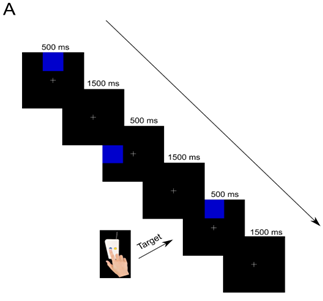
\includegraphics[clip, trim=0 0 0 15, width=\linewidth]{figs/nback.png} % Replace with your image path
        \subcaption{NBack FMRI task. } \label{fig:a}
    \end{minipage}
    \hspace{0.1\textwidth}
    \begin{minipage}{0.4\textwidth}
        \centering
        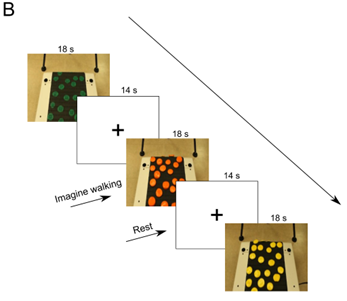
\includegraphics[clip, trim=0 0 0 15, width=\linewidth]{figs/imagery.png} % Replace with your image path
        \subcaption{Motor Imagery fMRI task.} \label{fig:b}
    \end{minipage}
    \caption{A) Schematic of example of a 2-back working memory task trial. Spatial targets appear for 500 ms and each target is separated by a 1500 ms interstimulus interval. B) Presentation of uneven terrain treadmill images during imagined walking trials. Colored images of the treadmill are displayed for 18 seconds per trial and with 14 seconds of rest between trials.}
    \label{fig:fmriTasks}
\end{figure}


\subsubsection{Motor imagery of uneven terrain walking}
As a part of the Mind in Motion study, participants performed treadmill walking on uneven terrains in a separate session, prior to undergoing MR neuroimaging \citep{Downey2022}. Uneven terrain treadmill walking could have been completed once or twice prior to the motor imagery session in the MRI scanner. 
% Table XX in the Result section shows participant demographics and their prior exposure to uneven terrain walking. 
Uneven terrains were created by adding foam disks to the treadmill belt. Terrain unevenness was modified by increasing the height and number of the discs \citep{Voloshina2013, Downey2022}. We created four levels of unevenness (Flat, Low, Medium, and High terrain unevenness). The Flat condition had flat, green circles painted onto the treadmill belt (i.e., normal walking). The Low condition had yellow-colored 1.3 cm-high disks. The Medium condition had orange-colored disks of two heights: 50\% were 1.3 cm and 50\% were 2.5 cm. The High condition had red-colored disks of three heights: 20\% were 1.3 cm, 30\% were 2.5 cm, and 50\% were 3.8 cm.

During the MR session, participants were instructed to imagine themselves walking on the uneven terrain treadmill belts. They performed two runs of imagined walking while fMR images were acquired in the scanner. They were shown pictures of the treadmill that they had previously walked on with the colored disks, from a first-person point of view (Fig 1 Panel B). While the picture is shown, participants were instructed to imagine walking on the treadmill, as they did during the prior walking visit. The four uneven terrain walking conditions were presented pseudorandomly. Within each run, uneven terrain conditions were presented twice for 18 seconds each, with 15 seconds of rest between the conditions. This resulted in a total of 288 seconds of imagined walking (2 runs X 4 uneven terrain conditions X 2 stimuli X 18 seconds stimulus presentation). At the start of each run, a brief message was displayed for 4.5 seconds, indicating the upcoming condition.

After the motor imagery task was completed, participants also completed a vividness of motor imagery questionnaire (VMIQ; \citealp{Isaac1986}), which asked them to self-report how well they were able to imagine themselves walking on the different uneven terrain treadmill conditions as the treadmill images were displayed. The VMIQ uses a rating scale ranging from 1 to 5, with 1 being “perfectly clear and vivid” imagery of the movement and 5 being “no image at all” of the movement.

\subsection{MR Image Processing}
\subsubsection{Whole brain preprocessing}
Preprocessing and data analyses were performed using the Statistical Parametric Mapping 12 software (SPM12; www.fil.ion.ucl.ac.uk/spm) implemented in MatLab (MathWorks Inc). Preprocessing steps included slice timing correction, realignment of functional volumes to participant-specific mean functional image, and reslicing to correct for volume-to-volume head motion. We also used the Artifact Detection Tool (ART, www.nitrc.org/projects/artifact\_detect/). Within each run, a volume was considered an outlier (and covaried out) if the participant’s composite movement was equal to or greater than 2.5 mm. fMR images were normalized to Montreal Neurologic Institute 152 (MNI152) standard space using Advanced Normalization Tools (ANTs) \citep{Avants2011} in a multi-step procedure:
\begin{itemize}
    \item the T1 images were skull stripped using ImCalc (SPM12);
    \item participant-specific T1 templates were created;
    \item participant-specific mean fMRI templates were created for each individual run;
    \item the mean fMRI templates were coregistered to the T1 participant-specific templates with rigid and affine registration;
    \item the T1 templates were normalized to MNI152 standard space with rigid, affine, and SyN registration;
    \item we concatenated these warps into a single flowfield (preprocessed fMRI native space image to mean fMRI template; mean fMRI template to T1 template; T1 template to MNI space);
    \item the resulting warp parameters were applied to each fMRI run to normalize the functional images to standard space (MNI) in one step.
\end{itemize}

After normalization to MNI space, the voxel size was 2×2×2 mm$^3$. Finally, the normalized fMRI images were spatially smoothed with a 4-mm full-width half-maximum Gaussian kernel.

\subsubsection{Cerebellar preprocessing}
Custom cerebellar preprocessing was performed by using portions of both the CEREbellum Segmentation (CERES; \citealp{Romero2017}) pipeline and ANTs \citep{Avants2011} to normalize each subject's cerebellum to the Spatially Unbiased Infratentorial Template (SUIT; \citealp{Diedrichsen2006, Diedrichsen2009}). We used the CERES pipeline to segment the cerebellum from each T1-weighted image. We then created binary gray matter, white matter, and full cerebellar masks from the CERES native space output and masked the unwarped-realigned fMRI data to extract the functional data for the cerebellum. We then normalized the structural cerebellum to a custom SUIT template using ANTs \citep{Avants2011} and applied those transformation warps to the functional cerebellar image individually for each participant.

\subsection{fMRI Data Analyses}
We calculated participant-level (1st level) brain activity during the motor imagery and working memory tasks from our preprocessed images. We produced four statistical parametric maps (SPM) for each participant to determine task-based brain activity compared to rest on a voxel-by-voxel basis using the following SPM contrasts for the n-back task: 0-back > rest, 1-back > rest, 2-back > rest, and 3 > rest; and the motor imagery task: Flat > rest, Low > rest, Med > rest, and High > rest.

\subsection{Region of Interest (ROI) analyses}
First level contrasts (task > rest) were used to extract mean brain activity beta values from the ROIs listed below. Mean beta was extracted as a mean of the betas across all the voxels in a given ROI. We created ROIs for the n-back task using the neurosynth meta-analysis of 1091 published studies on working memory function \citep{Yarkoni2011}.

We then use R studio (R 4.1.0) to perform linear mixed-model analyses to determine potential interactions between age and task difficulty (condition) across each ROI for the N-back and motor imagery tasks, and also across each ISI for the N-back task.


\subsubsection{Whole brain and cerebellum analyses}
We performed whole brain and cerebellum exploratory analyses to determine brain regions activated by motor imagery of uneven terrain walking. Second level contrasts were created to examine overall activation by the motor imagery task from the first level contrasts (task > rest) across each age group (older adults were not split into separate groups based on mobility function for these analyses). We tested the main effect and interaction effect to identify regions that increase in task-based brain activity as the motor imagery task complexity increases across age groups. We tested whole brain and cerebellum activations for condition effects (High>Med>Low>Flat), age effects (OA>YA), and condition by age interaction effects. The condition by age interaction was based on the CRUNCH-related increase of brain activity, so the contrast weights reflected a greater slope increase for older adults than young adults and a plateau in older adult brain activity at higher task difficulty, which resulted in a contrast with the following weights (contrast weights across age and condition: YAFlat=1; YALow=2; YAMed=3; YAHigh=4;  OAFlat=2; OALow=4; OAMed=8; OAHigh=8). 

For whole brain analysis (cerebrum only), we masked the cerebellum. For the cerebellum images, we used outputs from our custom cerebellum preprocessing, which normalizes the cerebellum to the SUIT template. We used the Sandwich Estimator Toolbox (SwE; \citealp{Guillaume2014}) for these exploratory analyses. The SwE toolbox defaults were used, except for nonparametric wild bootstrap with 999 iterations \citep{Guillaume2015} and threshold-free cluster enhancement (TFCE; \citealp{Smith2009}). Nonparametric estimation avoids parametric (e.g., random field theory) distribution assumptions. TFCE produces results in which voxel-wise values represent the amount of cluster-like local spatial support. TFCE is favorable as it does not require an arbitrary cluster-forming threshold and it is more sensitive compared with other thresholding methods \citep{Smith2009}. Significance was determined at $p<0.05$, family-wise error (FWE) corrected for multiple comparisons.

\subsection{Behavioral analysis}
\subsubsection{N-back task}
We calculated d prime for the n-back task. D prime was calculated as the difference between Z transform of hit rate and the false alarm rate. D prime was calculated for each of the n-back conditions, across each subject.

\subsubsection{Motor Imagery task}
We also calculated the average self-reported quality of imagery from our custom vividness of motor imagery questionnaire. Vividness scores from the questionnaire were averaged for each of the motor imagery conditions across our sample of older and younger adults.

\subsubsection{Cross task correlation}
We calculated CRUNCH scores for the N-back task, within the predetermined neurosynth-derived ROIs. CRUNCH scores were calculated as the task difficulty level at which the “ceiling” in brain activity was hit. Within participants who exhibit CRUNCH ceilings in the N-back task, we determined if they also reached a CRUNCH ceiling within the activated brain regions determined by the whole brain and cerebellum analysis during motor imagery.

\begin{table}[h!]
\caption{Participant demographics.}\label{tab:demographics}
\centering
\begin{tabular}{lccccc}
\textbf{} & \textbf{Age (yrs)} & \textbf{Sex} & \textbf{MoCA Score} & \textbf{400m Walk (s)} & \textbf{SPPB} \\ 
\textbf{YA} & $23.0 \pm 3.4$ & 11/22 males & $28.1 \pm 1.5$ & $345.8 \pm 51.9$ & N/A \\ 
\textbf{OA} & $74.9 \pm 6.3$ & 15/38 males & $26.9 \pm 1.6$ & $389.8 \pm 90.8$ & $10.0 \pm 1.8$ \\ 
\textbf{HOA} & $73.8 \pm 5.2$ & 13/27 males & $27.1 \pm 1.5$ & $360.5 \pm 62.9$ & $11.0 \pm 0.9$ \\ 
\textbf{LOA} & $77.6 \pm 8.1$ & 2/11 males & $26.4 \pm 1.7$ & $461.7 \pm 110.6$ & $7.7 \pm 1.2$ \\ 
\end{tabular}
\end{table}


\section{Results}	

Overall The Nback results 
All participants completed each of the tasks analyzed in this manuscript, including functional MRI tasks and cognitive (MoCA) and physical (400m walk) assessments, excluding younger adults for SPPB. The summary results of the cognitive and physical assessments are shown in Table \ref{tab:demographics}. In general, younger adults scored better on the MoCA and 400-m walk than HFOA, and HFOA scored better on 400m walk and SPPB than LFOA.  

\subsection{Behavioral Results}
\subsubsection{NBack Working Memory Task}

The NBack behavior performance exhibited several significant findings. The short ISI shows significant differences for Dprime between group and n-back condition, individually, but no significant interaction between the two factors (Table \ref{tab:nback_dprime_results}). The long ISI exhibits a significant difference between groups and n-back, as well as their interaction (Table \ref{tab:nback_dprime_results}). Figure \ref{fig:dprime} provides visualization of the participant averages of Dprime for each of the conditions.

\begin{table}[h!]
\caption{Nback Dprime statistical test results for Short and Long ISI conditions. Significance codes: 0 ‘***’ 0.001 ‘**’ 0.01 ‘*’ 0.05 ‘.’ 0.1 ‘ ’ 1.}
\label{tab:nback_dprime_results}
\centering
\begin{tabular}{llrrrrr}
\toprule
\multirow{2}{*}{}               & \multirow{2}{*}{}          & \textbf{Sum Sq  } &  \textbf{Mean Sq} & \textbf{NumDF} & \textbf{DenDF} & \textbf{Pr(>F)}          \\ 

\midrule
\multirow{3}{*}{\textbf{Short ISI}} 
                                & \textbf{Grp}              & 8.139            & 4.0693            & 2               & 57.227          & 2.58e-05 ***             \\
                                & \textbf{Cond}             & 72.309           & 24.1032           & 3               & 169.377         & < 2.2e-16 ***            \\
                                & \textbf{Grp:Cond}         & 2.004            & 0.334             & 6               & 169.063         & 0.3957                   \\ 
\midrule
\multirow{3}{*}{\textbf{Long ISI}}
                                & \textbf{Grp}              & 11.596           & 5.7978            & 2               & 57              & 4.51e-06 ***             \\
                                & \textbf{Cond}             & 36.274           & 12.0915           & 3               & 171             & < 2.2e-16 ***            \\
                                & \textbf{Grp:Cond}         & 7.241            & 1.2068            & 6               & 171             & 0.0052 **                \\ 
\bottomrule
\end{tabular}
\end{table}


\begin{figure}[h]
    \centering
    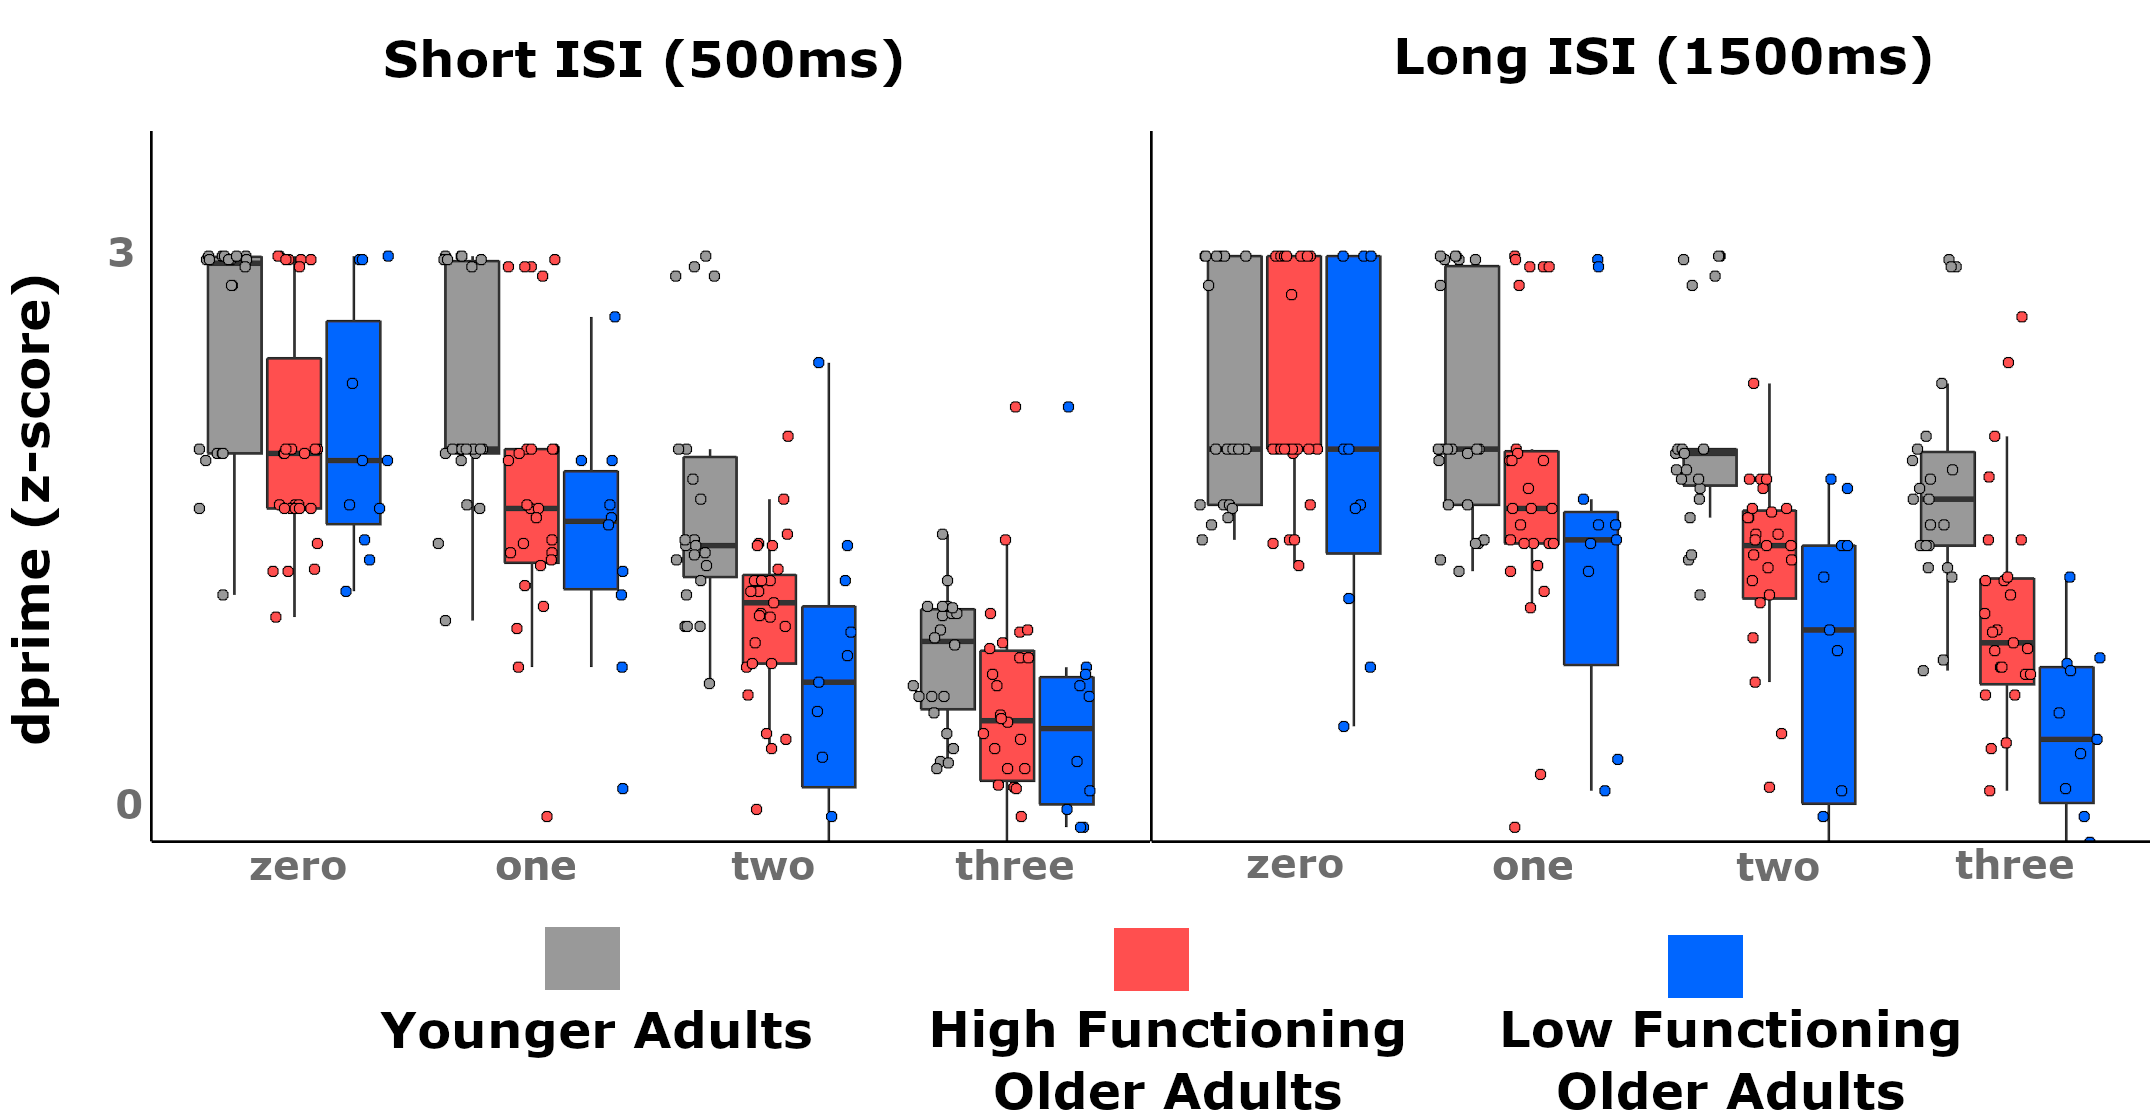
\includegraphics[clip, trim=0 0 0 0, scale=0.75]{figs/nback_dprime.png} % Replace with your image path
    \caption{Behavioral results for Nback short and long ISI. Dprime is displayed on y-axis, groups are color coded, and the means for each participant are displayed as smaller dots within the whisker plot. }
    \label{fig:dprime}
\end{figure}

\subsubsection{Motor Imagery Task}
Participants reported good visualization during the imagined walking task. XX Figure XX 

\newpage

\subsection{Region of Interest (ROI) analyses}
\subsubsection{N-back working memory task}
Table \ref{tab:nback_roi_results} displays LME analysis results for group by condition interactions, for each ISI and ROI post-hoc comparisons for significant interactions. The right and left DLPFC were significantly different between conditions for both short and long ISI (p < .001). Only the left DLPFC with short ISI exhibited an interaction between group and condition (p < .01). Figure \ref{fig:ROI_nbackfmriTasks} displays the beta values for each group, across the difficulty levels (conditions) for the left and right DLPFC. The ACC did not exhibit any significant results.

\begin{table}[h!]
\centering
\caption{Results of statistical tests for ACC, R DLPFC, and L DLPFC across Short and Long ISI conditions for the Nback fMRI task.}
\label{tab:nback_roi_results}
\begin{tabular}{llrrrr}
\toprule
\textbf{ISI}   & \textbf{Region} & \textbf{F value} & \textbf{Pr(>F)} & \textbf{Effect} \\ 
\midrule
Short          & ACC            & 1.4246           & 0.208           & Grp:Cond        \\
               & R DLPFC        & 16.5426          & \textbf{1.75e-09***} & Cond        \\
               & L DLPFC        & 16.0309          & \textbf{3.14e-09***} & Cond        \\
               & L DLPFC        & 2.9955           & \textbf{0.0083**}  & Grp:Cond        \\
Long           & ACC            & 1.6118           & 0.147           & Grp:Cond        \\
               & R DLPFC        & 30.5194          & \textbf{7.47e-16***} & Cond        \\
               & L DLPFC        & 22.186           & \textbf{3.49e-12***} & Cond        \\
\bottomrule
\multicolumn{5}{l}{Signif. codes: 0 ‘***’ 0.001 ‘**’ 0.01 ‘*’ 0.05} 
\end{tabular}
\end{table}



\begin{figure}[h!]
    \centering
    \begin{minipage}{0.48\textwidth}
        \centering
        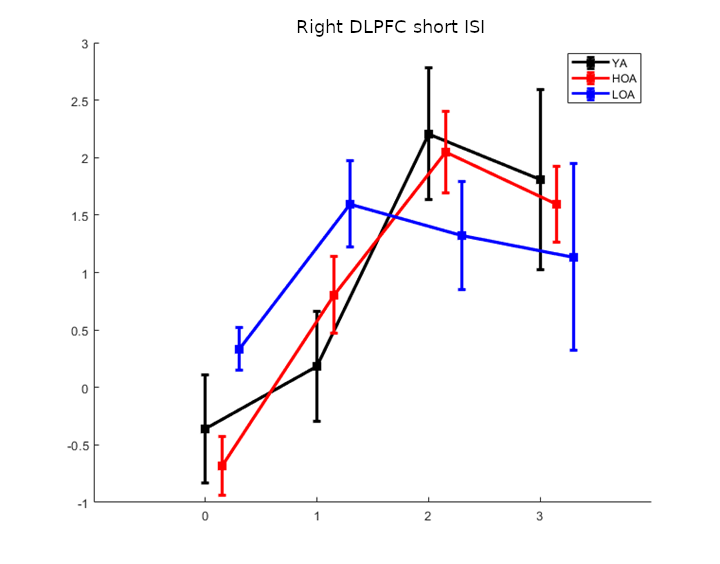
\includegraphics[clip, trim=0 0 0 0, width=\linewidth]{figs/Nback500_rdlpfc_neurosynth.png} % Replace with your image path
        \subcaption{Short ISI R DLPFC ROI beta values across NBack conditions. } \label{fig:a}
    \end{minipage}
    % \hspace{\textwidth}
    \begin{minipage}{0.48\textwidth}
        \centering
        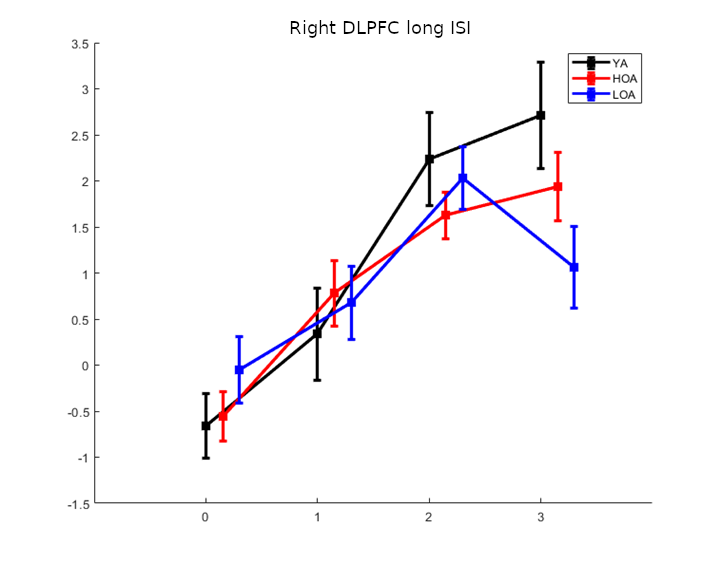
\includegraphics[clip, trim=0 0 0 0, width=\linewidth]{figs/Nback1500_rdlpfc_neurosynth.png} % Replace with your image path
        \subcaption{Long ISI R DLPFC ROI beta values across NBack conditions.} \label{fig:b}
    \end{minipage}
    \begin{minipage}{0.48\textwidth}
        \centering
        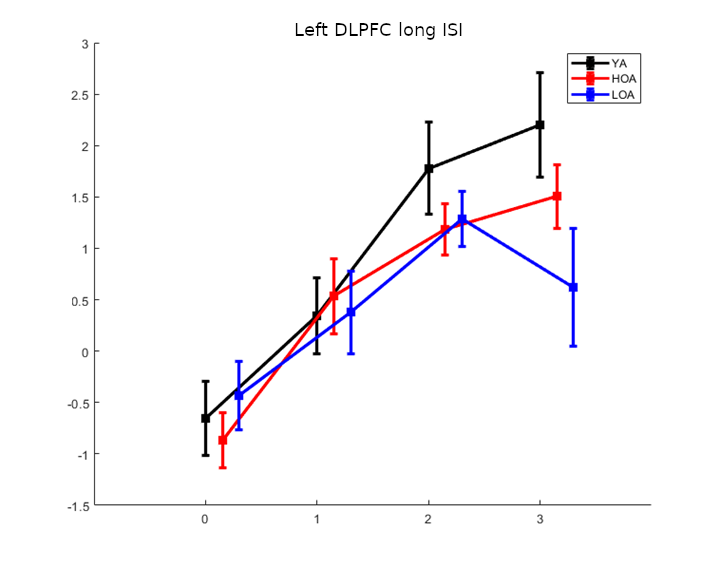
\includegraphics[clip, trim=0 0 0 0, width=\linewidth]{figs/Nback1500_ldlpfc_neurosynth.png} % Replace with your image path
        \subcaption{Long ISI L DLPFC ROI beta values across NBack conditions.} \label{fig:b}
    \end{minipage}
    \caption{Display of the significant ROIs during the N-back task.}
    \label{fig:ROI_nbackfmriTasks}
\end{figure}

\clearpage


\subsubsection{Motor Imagery of walking task}
The chosen ROIs (ACC and right and left DLPFC) did not show any significant results across condition or group for the motor imagery fmri task.


\subsection{Whole brain exploratory analyses}
\subsubsection{Cerebrum activation}
There were several significant results stemming from the whole brain analysis with age and condition used as co-variates. Table \ref{tab:MI_cerebrum_interaction} shows the coordinate clusters and their signficance level, and Figure \ref{fig:MotorImagery_cerebrum_interaction} shows the clusters within a brain template. The largest and most statistically significant cluster was the left lingual area (pFWE-corr < .001; kE 14493), which included left Middle Occiptal and the right Calcarine area. The next largest cluster involved left Paracentral Lobule, left Supplementary Motor, and left Superior Frontal areas (p< .005; kE 2620). Other significant clusters include right precentral area, and the left inferior frontal Triangular area. 

\begin{figure}[h]
    \centering
    \begin{minipage}{0.55\textwidth}
        \centering
        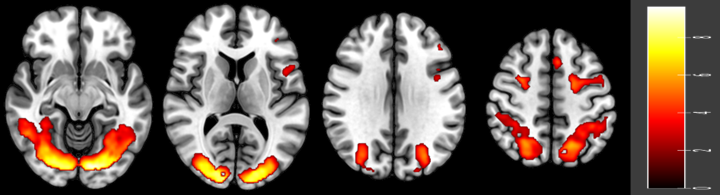
\includegraphics[clip, trim=0 0 0 0, width=\linewidth]{figs/brainSlice_Interaction.png} % Replace with your image path
        \subcaption{Cerebrum age x condition interaction results (slide -10 10 30 50). } \label{fig:a}
    \end{minipage}
    % \hspace{\textwidth}
    \begin{minipage}{0.35\textwidth}
        \centering
        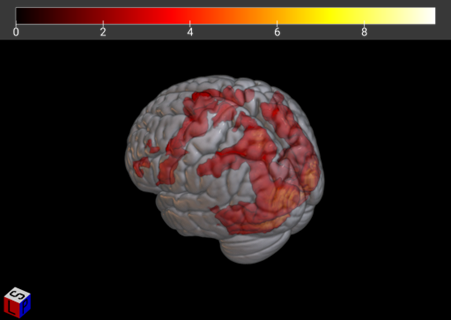
\includegraphics[clip, trim=0 0 0 0, width=\linewidth]{figs/brain_Interaction.png} % Replace with your image path
        \subcaption{Cerebrum age x condition interaction results (whole brain).} \label{fig:b}
    \end{minipage}
    \caption{Brain activation showing age by condition interactions across the brain cerebrum. Motor imagery of uneven terrain walking required increased cortical activation for older adults, compared to younger adults in the areas highlighted. }
    \label{fig:MotorImagery_cerebrum_interaction}
\end{figure}

\begin{table}[h]
\centering
\caption{Brain activation showing age by condition interactions across the brain cerebrum. Motor imagery of uneven terrain walking required increased cortical activation for older adults, compared to younger adults in the areas highlighted. }
    \label{tab:MI_cerebrum_interaction}
\begin{tabular}{lllllll}

               & \multicolumn{2}{l}{TFCE-level} & \multicolumn{3}{c}{MNI coordinates (mm)} &  \\
& pFWE-corr        & kE          & X            & Y           & Z           &  \\ 
Left Lingual                             & 0.001            & 14493       & -18          & -84         & -12         &  \\
Left Middle Occipital                    &                  &             & -12          & -94         & 2           &  \\
Right Calcarine                          &                  &             & 14           & -94         & 6           &  \\
Left Paracentral Lobule                  & 0.005            & 2620        & -14          & -24         & 70          &  \\
Left Supplementary Motor                 &                  &             & -6           & -2          & 70          &  \\
Left Superior Frontal                    &                  &             & -22          & -6          & 54          &  \\
Right Precentral                         & 0.028            & 154         & 28           & 0           & 50          &  \\
\cellcolor[HTML]{D0CECE}                 &                  &             & 22           & -12         & 54          &  \\
Left Inferior Frontal Triangular         & 0.04             & 107         & -46          & 46          & 2           &  \\
Left Inferior Frontal Triangular         &                  &             & -38          & 40          & 4           &  \\
Left Inferior Frontal Triangular         & 0.044            & 29          & -42          & 28          & 26          &  
\end{tabular}
\end{table}


\subsubsection{Cerebellum activation}
Table \ref{tab:MotorImagery_cerebellum_interaction} and Figure \ref{fig:MotorImagery_cerebellum_interaction} display the significant results within the cerebellum with age and condition used as co-variates. The right cerebellum 8 area had the largest significant cluster (kE=580), which included clusters that covered parts of Crus I and cerebellum module 6. Several smaller individual clusters were presetn in Cerebellum module 9. 


\begin{figure}[ht]
    \centering
    \begin{minipage}{0.55\textwidth}
        \centering
        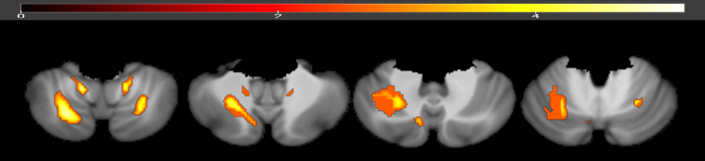
\includegraphics[clip, trim=0 0 0 0, width=\linewidth]{figs/cerebellumSlice_Interaction.png} % Replace with your image path
        \subcaption{Cerebellum age x condition interaction results (slide -10 10 30 50). } \label{fig:a}
    \end{minipage}
    % \hspace{\textwidth}
    \begin{minipage}{0.35\textwidth}
        \centering
        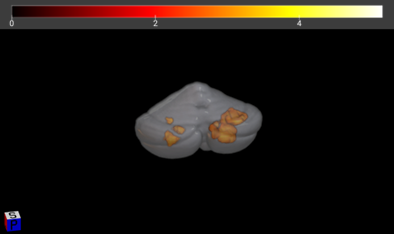
\includegraphics[clip, trim=0 0 0 0, width=\linewidth]{figs/cerebellum_Interaction.png} % Replace with your image path
        \subcaption{Cerebellum age x condition interaction results (whole brain).} \label{fig:b}
    \end{minipage}
    \caption{Brain activation showing age by condition interactions across the cerebellum. }
    \label{fig:MotorImagery_cerebellum_interaction}
\end{figure}


\begin{table}[]
\centering
\caption{Results of statistical tests for cerebellum during motor imagery; age x condition. }
\label{tab:MotorImagery_cerebellum_interaction}
\begin{tabular}{lllllll}

         & \multicolumn{2}{c}{TFCE-level} & \multicolumn{3}{c}{MNI coordinates (mm)} &  \\
  & pFWE-corr         & kE         & X            & Y           & Z           &  \\ 
Right Cerebellum 8                        & 0.004             & 580        & 24           & -66         & -43         &  \\
Right Cerebellum Crus I                   &                   &            & 34           & -68         & -29         &  \\
Right Cerebellum 6                        &                   &            & 26           & -62         & -31         &  \\
Right Cerebellum 9                        & 0.017             & 47         & 16           & -54         & -43         &  \\
Left Cerebellum 9                         & 0.02              & 42         & -16          & -52         & -43         &  \\
Left Cerebellum 9                         &                   &            & -18          & -44         & -47         &  \\
Left Cerebellum 6                         & 0.038             & 11         & -26          & -60         & -27         &  \\
Left Cerebellum 8 & 0.025             & 65         & -24          & -64         & -45         &  
\end{tabular}
\end{table}


\section{Discussion }
Overall, our hypothesis that there would be an overlap in functionality and presenece of a CRUNCH point within the ROIs of anterior cingulate and bilateral DLPFC during cognitive and imagined motor tasks proved incorrect.

\subsection{N-back Task Results}
The Nback results from the ROI analysis proved the task challenging enough to exhibit the hypothesized CRUNCH point, however, the same ROIs during the motor imagery task did not show these patterns.
The whole brain analysis for the motor imagery task did present with multiple brain regions exhibiting the CRUNCH behavior, but primarily in occipital, supplementary motor, and inferior frontal areas. 
These results will help us unpack the heterogeneous effects of aging.

The Nback results indicated that older adults with higher physical function demonstrated similar brain activation patterns compared to younger adults. 
The lower functioning older adults reached their CRUNCH point during the Nback earlier than the higher functioning older adults. Considering the lower functioning older adults were categorized based on physical traits (SPPB score), performed worse on the Nback task, and also exhibited earlier CRUNCH points, this is compelling evidence that there is a link between physical and cognitive function.

\subsection{Motor Imagery Task Results}
The motor imagery tasks did not present any results with the chosen ROIs, therefore we pursued an exploratory whole brain analysis to uncover what, if any, brain regions were exhibiting the type of behavior we expected given the results of the Nback task. The whole brain analyses of motor imagery does show that older adults utilize greater brain resources than younger adults, furthermore, they also utilized cerebellar regions (see Results Section @). 
Primarily occipital, supplementary motor, and inferior frontal areas exhibited the expected group and condition effects. 
In the cerebellum, modules 6, 8, and 9 exhibited the same effects.

These findings suggest that while older adults engage additional neural resources, including cerebellar areas, to compensate for task demands, the expected overlap in anterior cingulate and DLPFC functionality was absent. Instead, the results highlight the heterogeneous effects of aging on neural activation and the distribution of compensatory mechanisms across different brain regions.


\subsection{Implications}
The lack of results for the ROI analysis in the motor imagery task is surprising given the apparent link between physical and cognitive performance observed with the lower physical functioning older adults in the N-back. However, it appears it is more nuanced than that. The observed link—lower-functioning older adults performing worse on the N-back task and exhibiting earlier CRUNCH points—may not reflect a direct overlap in neural resources. Instead, it may indicate a systemic degradation affecting both peripheral and central systems, however it is likely more nuanced than that.

The current results align closely with the notion of systemic degradation described in Clark et al. (2015); however, the proposed shift from lower-level (spinal) control to higher-level (cerebral/executive) control for motor tasks in older adults was not observed. It is possible that neural compensation, such as the utilization of frontal resources, in older adults during motor tasks is primarily required during actual walking due to the increased complexity of actually performing the task versus imagining. Mounting evidence supports increased frontal activation of older adults compared to younger adults during walking (@refs). The sensory input alone from stimulating the soles of the feet and moving the large muscle groups in the legs and controlling balance could be enough to overload the lower level neural mechanisms in older adults, compared to imagining the movement. There is also an emotional component to walking (@ref), which is linked to the risk of falling, which would likely utilize neural resources. During imagined walking, there is no actual risk of falling, therefore those neural resources may not be utilized. Furthermore, we suspect that the frontal shift of a lower level task such as walking, and even imagined walking, could be exacerbated in multi-tasking situations—for example, conversing with someone or navigating a complex environment. These secondary tasks (e.g., visual or linguistic processing), which are superimposed on the primary task of walking, may recruit brain areas highlighted in the whole-brain motor imagery task, such as visual and lingual regions. This additional demand might then necessitate the involvement of more executive brain areas, including the anterior cingulate cortex (ACC) and DLPFC. This holistic perspective underscores the importance of considering both central and peripheral factors when examining age-related changes in neural compensation and motor-cognitive interactions, and also identifies gaps in understanding which can be addressed in future study designs.



\subsection{Limitations/Considerations}
The primary consideration is that we are using a motor imagery task as a proxy for actually walking because of the requirements associated with MRI. MRI enables us to look into the deepest parts of the brain with millimeter accuracy, which comes at a cost of temporal resolution, as well as susceptibility of movement artifacts. So tasks that are performed while simultaneously imaging their brain with MRI must enable a completely immobile head. There are several experiments aiming to elucidate the similarities and differences between imagined for actual movement (@refs), but there will always be the missing sensory information that is provided by actual movement that imagined movement lacks. Additionally, there are varying degrees of the ability to imagine, and there are also biases with self-rating that ability (@refs). So despite participants reporting decent ability to imagine (or recall) themselves walking on the uneven terrain, we do not have a mechanism to prove that their report is accurate.




\section{Conclusion}
This study provides valuable insights into the complex interplay between physical and cognitive function in older adults, particularly through the lens of neural compensation and CRUNCH-related patterns. While the N-back task results support a link between physical and cognitive performance, the motor imagery task highlights the heterogeneous nature of compensatory neural mechanisms. The absence of anticipated CRUNCH-related activity in the anterior cingulate and DLPFC during motor imagery suggests a more systemic degradation, rather than localized neural reorganization. However, it must be considered that imagined walking may not provide the necessary demands on the neural resources to observe the consistently reported over activation of frontal areas in older compared to younger adults during actual walking. These findings underscore the importance of a holistic approach to understanding age-related neural changes and highlight areas for further investigation to improve interventions aimed at maintaining cognitive and motor function in older populations.



\clearpage
% Statements and Declarations
% \begin{declarations}
\section*{Statements and Declarations}
On behalf of all authors, the corresponding author states that there are no conflicts of interest.

\section*{Data Availability}
Data from the current study are available from the corresponding author on reasonable request. All requests will be reviewed by the University of Florida.

\section*{Acknowledgements}
We thank all the participants for their time in the study and the research coordinator staff for participant recruitment.

\section*{Funding}
This work was supported by: National Institutes of Health under award numbers: NIA U01AG061389 and NIA T32AG062728. A portion of this work was performed in the McKnight Brain Institute at the National High Magnetic Field Laboratory’s Advanced Magnetic Resonance Imaging and Spectroscopy (AMRIS) Facility, supported by National Science Foundation Cooperative Agreement No. DMR-1644779 and the State of Florida. Additionally, this work was supported in part by NIH award S10 OD021726 for High End Instrumentation.
% s\end{declarations}


%% Loading bibliography style file
%\bibliographystyle{model1-num-names}
\bibliographystyle{cas-model2-names}

% Loading bibliography database
\bibliography{library}

\clearpage

% \appendix
\section{Supplementary Info}
% Appendix sections are coded under \verb+\appendix+.



\begin{table}[]
\caption{Neurosynth based ROIs for N-back.}\label{tab:ROI_neurosynth}
\begin{tabular}{lllll}
\textbf{Brain Region}                & \multicolumn{3}{l}{\textbf{MNI Coordinates (mm)}} & \textbf{Size (mm3)} \\
                                     & \textit{X}      & \textit{Y}     & \textit{Z}     &                     \\
Left Dorsolateral Prefrontal Cortex  & -               & -              & -              & 7616                \\
Right Dorsolateral Prefrontal Cortex & -               & -              & -              & 6472                \\
Anterior Cingulate Cortex            & -               & -              & -              & 32776              
\end{tabular}
\end{table}

\begin{table}[]
\caption{For motor imagery of uneven terrain walking, we used ROIs based on previous studies of motor imagery of walking and CRUNCH. Spherical ROIs were created at MNI coordinates from (Allali et al. 2014 and Gerver et al. 2020). }\label{tab:ROI_coords}
\begin{tabular}{lllll}
\textbf{Brain Region}         & \multicolumn{3}{l}{\textbf{MNI Coordinates (mm)}} & \textbf{Size (mm3)} \\
                              & \textit{X}      & \textit{Y}     & \textit{Z}     &                     \\
Left Hippocampus              & -31             & -24            & -12            & 152                 \\
Right Hippocampus             & 32              & -24            & -9             & 152                 \\
Supplementary Motor Area      & 0               & -6             & 63             & 648                 \\
Left Inferior Occipital Lobe  & -20             & -100           & -6             & 648                 \\
Right Inferior Occipital Lobe & 19              & -98            & -6             & 648                 \\
Left Paracentral Lobule       & 9               & -36            & 75             & 648                 \\
Right Paracentral Lobule      & 10              & 40             & 72             & 648                 \\
Left Premotor Cortex          & 30              & 4              & 58             & 648                 \\
Right Premotor Cortex         & -26             & 2              & 58             & 648                
\end{tabular}

\end{table}

\begin{longtable}{|p{0.95\linewidth}|}
\hline
\rowcolor[HTML]{C0C0C0} 
\textbf{Criteria} \\ 
\hline
\textbf{Inclusion Criteria:}
\begin{itemize}
    \item Community-dwelling men and women:
        \begin{itemize}
            \item Aged 70+ years for White, Non-Hispanic participants.
            \item Aged 65+ years for participants of other races and ethnicities.
            \item Aged 20–40 years.
        \end{itemize}
    \item Short Physical Performance Battery (SPPB):
        \begin{itemize}
            \item SPPB < 10 for moderate to low-functioning older adults (45\% of sample with SPPB < 8).
            \item SPPB $\geq$ 10 for high-functioning older adults.
        \end{itemize}
    \item Must complete a 400m walk test within 15 minutes without assistance (a cane is allowed, but not a walker).
    \item Willingness to undergo all testing procedures.
    \item English-speaking participants only.
    \item Willingness to enroll for 1.25–3 years, depending on enrollment date.
\end{itemize} \\ 
\hline
\textbf{Exclusion Criteria:}
\begin{itemize}
    \item Significant medical event requiring hospitalization in the past 6 months (e.g., fracture).
    \item Severe visual impairment (corrected visual acuity <20/40).
    \item Not MRI-eligible (e.g., due to metal implants).
    \item Clinically diagnosed vestibular dysfunction.
    \item Unable or unwilling to perform uneven terrain tasks without assistive devices.
    \item Chest pain or severe shortness of breath during physical stress.
    \item History of stroke or traumatic brain injury.
    \item Diagnosis of dementia or cognitive impairment:
        \begin{itemize}
            \item Score of 17 on the modified Telephone Inventory for Cognitive Status (TICS).
        \end{itemize}
    \item Major ADL disability (e.g., inability to feed, dress, bathe).
    \item Lower extremity pain from osteoarthritis limiting mobility.
    \item Diagnosis or treatment for rheumatoid arthritis.
    \item Lives in a nursing home (assisted or independent living not excluded).
    \item Receiving physical therapy for gait or lower extremity issues.
    \item Neuromuscular or overt neurological disorders (e.g., Multiple Sclerosis, Parkinson’s Disease).
    \item Severe hearing loss or speech disorder preventing communication.
    \item Planned surgeries or hospitalizations (e.g., joint replacement, CABG).
    \item Severe pulmonary disease requiring supplemental oxygen.
    \item Terminal illness as determined by a physician.
    \item Severe cardiac disease:
        \begin{itemize}
            \item NYHA Class III/IV CHF, significant aortic stenosis, cardiac defibrillator, uncontrolled angina.
        \end{itemize}
    \item Planning to move out of the area or be away for >6 months.
    \item Other significant medical conditions affecting safety/compliance (e.g., renal failure, psychiatric disorders).
    \item Use of walker or wheelchair.
    \item Failure to provide informed consent.
    \item Bloodwork abnormalities:
        \begin{itemize}
            \item Transaminases >2x upper limit of normal.
            \item Hemoglobin <10 g/dL.
        \end{itemize}
\end{itemize} \\ 
\hline
\textbf{Temporary Exclusion Criteria:}
\begin{itemize}
    \item Clinically significant abnormalities in blood chemistry.
    \item Severe hypertension (SBP >200 mmHg, DBP >110 mmHg).
    \item Uncontrolled diabetes or hyperglycemia (fasting glucose >126 mg/dL or HbA1c >6.5\%).
    \item Other temporary conditions (e.g., sick spouse, bereavement, recent move).
    \item Risk factors identified during medical history at enrollment.
\end{itemize} \\
\hline
\caption{Inclusion, Exclusion, and Temporary Exclusion Criteria for Participant Enrollment}
\label{tab:criteria}
\end{longtable}



\begin{figure}[ht]
    \centering
    \begin{minipage}{0.48\textwidth}
        \centering
        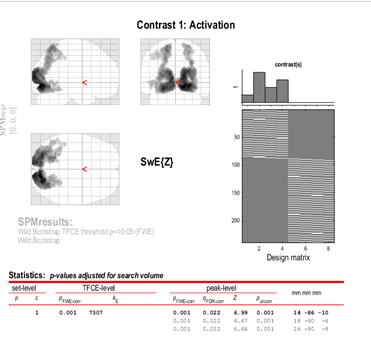
\includegraphics[clip, trim=0 0 0 0, width=\linewidth]{figs/YA_spm.png} % Replace with your image path
        \subcaption{XX: Slices: -20 -10 0; 10 20 30; 40 50 60; 70. } \label{fig:a}
    \end{minipage}
    % \hspace{\textwidth}
    \begin{minipage}{0.48\textwidth}
        \centering
        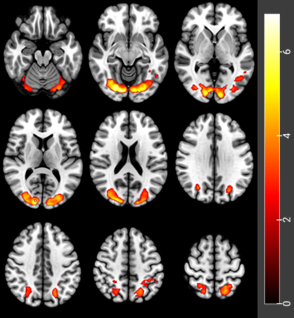
\includegraphics[clip, trim=0 0 0 0, width=\linewidth]{figs/YA_slice.png} % Replace with your image path
        \subcaption{XX: Slices: -20 -10 0; 10 20 30; 40 50 60; 70.} \label{fig:b}
    \end{minipage}
    \caption{XX: Slices: -20 -10 0; 10 20 30; 40 50 60; 70. }
    \label{fig:YA_slice}
\end{figure}



\begin{figure}[ht]
    \centering
    \begin{minipage}{0.48\textwidth}
        \centering
        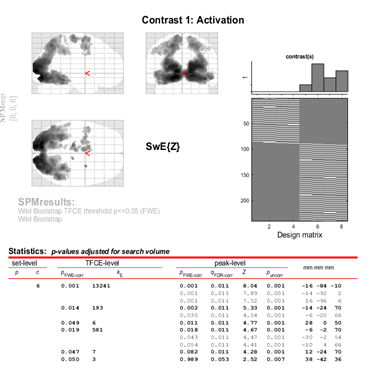
\includegraphics[clip, trim=0 0 0 0, width=\linewidth]{figs/OA_spm.png} % Replace with your image path
        \subcaption{XX: Slices: -20 -10 0; 10 20 30; 40 50 60; 70. } \label{fig:a}
    \end{minipage}
    % \hspace{\textwidth}
    \begin{minipage}{0.48\textwidth}
        \centering
        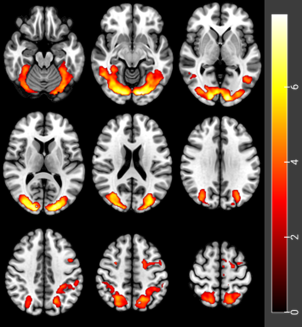
\includegraphics[clip, trim=0 0 0 0, width=\linewidth]{figs/OA_slice.png} % Replace with your image path
        \subcaption{XX: Slices: -20 -10 0; 10 20 30; 40 50 60; 70.} \label{fig:b}
    \end{minipage}
    \caption{XX: Slices: -20 -10 0; 10 20 30; 40 50 60; 70. }
    \label{fig:YA_slice}
\end{figure}

% Required packages: multirow, xcolor (use colortbl for Beamer presentations)
\begin{table}[h!]
\centering
\begin{tabular}{|c|l|c|c|c|c|c|}
\hline
\rowcolor[HTML]{D0D0D0} 
\textbf{Group}           & \textbf{Region}                 & \textbf{pFWE-corr} & \textbf{kE} & \textbf{X}   & \textbf{Y}  & \textbf{Z}  \\ \hline
                         & Right Lingual                  & 0.001             & 7307        & 14           & -86         & -10         \\ 
                         & Right Lingual                  &                   &             & 18           & -80         & -6          \\ 
\multirow{-3}{*}{\textbf{Young Adults}}  
                         & Right Fusiform                 &                   &             & 26           & -80         & -8          \\ \hline
                         & Left Lingual                   & 0.001             & 13241       & -16          & -84         & -10         \\ 
                         & Left Superior Occipital        &                   &             & -14          & -92         & 2           \\ 
                         & Right Calcarine                &                   &             & 16           & -96         & 6           \\ 
                         & Left Paracentral Lobule        & 0.014             & 193         & -14          & -24         & 70          \\ 
                         & Left Paracentral Lobule        &                   &             & -6           & -20         & 66          \\ 
                         & Right Precentral               & 0.049             & 6           & 28           & 0           & 50          \\ 
                         & Left Supplementary Motor Area  & 0.019             & 581         & -6           & -2          & 70          \\ 
                         & Left Mid Frontal               &                   &             & -30          & -2          & 54          \\ 
                         & Left Supplementary Motor Area  &                   &             & -10          & 4           & 66          \\ 
                         & Right Paracentral Lobule       & 0.047             & 7           & 12           & -24         & 70          \\ 
\multirow{-11}{*}{\textbf{Older Adults}} 
                         & \cellcolor[HTML]{EAEAEA}       & 0.05              & 3           & 38           & -42         & 36          \\ \hline
\end{tabular}
\caption{TFCE-level results with MNI coordinates for young and older adults.}
\label{tab:tfce}
\end{table}



\begin{figure}[ht]
    \centering
    \begin{minipage}{0.48\textwidth}
        \centering
        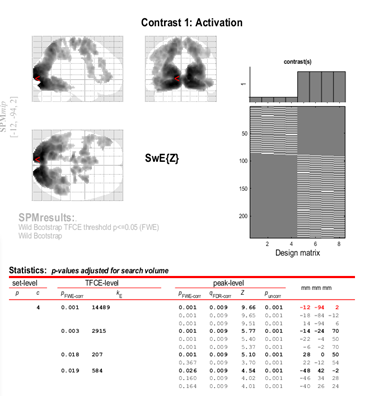
\includegraphics[clip, trim=0 0 0 0, width=\linewidth]{figs/OAYA_spm.png} % Replace with your image path
        \subcaption{XX:} \label{fig:a}
    \end{minipage}
    % \hspace{\textwidth}
    \begin{minipage}{0.48\textwidth}
        \centering
        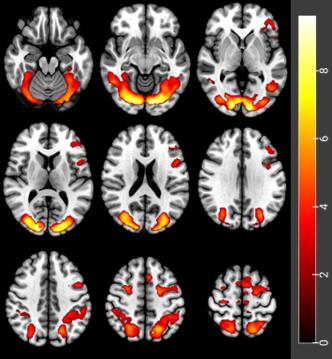
\includegraphics[clip, trim=0 0 0 0, width=\linewidth]{figs/OAYA_slice.png} % Replace with your image path
        \subcaption{XX: } \label{fig:b}
    \end{minipage}
    \caption{OA > YA}
    \label{fig:AgexCon_Slice}
\end{figure}


\begin{table}[h!]
\centering
\begin{tabular}{|l|c|c|c|c|c|}
\hline
\rowcolor[HTML]{D0D0D0} 
\textbf{Region}                     & \textbf{pFWE-corr} & \textbf{kE}  & \textbf{X}   & \textbf{Y}   & \textbf{Z}   \\ \hline
\textbf{Left Middle Occipital}      & 0.001             & 14489        & -12          & -94          & 2           \\ 
\textbf{Left Lingual}               &                   &              & -18          & -84          & -12         \\ 
\textbf{Right Calcarine}            &                   &              & 14           & -94          & 6           \\ \hline
\textbf{Left Paracentral Lobule}    & 0.003             & 2915         & -14          & -24          & 70          \\ 
\textbf{Left Supplementary Motor}   &                   &              & -22          & -4           & 50          \\ 
                                     &                   &              & -6           & -2           & 70          \\ \hline
\textbf{Right Paracentral}          & 0.018             & 207          & 28           & 0            & 50          \\ 
                                     &                   &              & 22           & -12          & 54          \\ \hline
\textbf{Left Inferior Frontal Orbital} & 0.019          & 584          & -48          & 42           & -2          \\ 
\textbf{Left Inferior Frontal Triangular} &             &              & -46          & 34           & 28          \\ 
                                     &                   &              & -40          & 26           & 24          \\ \hline
\end{tabular}
\caption{TFCE-level analysis results with MNI coordinates for regions of interest  for OA > YA.}
\label{tab:tfce_results}
\end{table}



\begin{figure}[ht]
    \centering
    \begin{minipage}{0.48\textwidth}
        \centering
        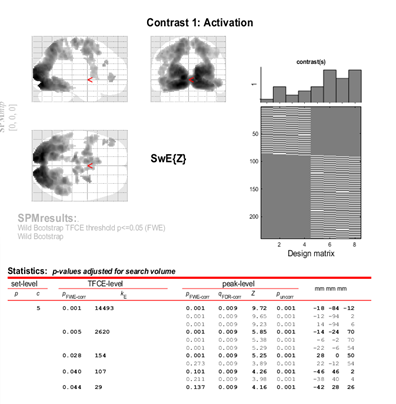
\includegraphics[clip, trim=0 0 0 0, width=\linewidth]{figs/AgeXCon_spm.png} % Replace with your image path
        \subcaption{XX:} \label{fig:a}
    \end{minipage}
    % \hspace{\textwidth}
    \begin{minipage}{0.48\textwidth}
        \centering
        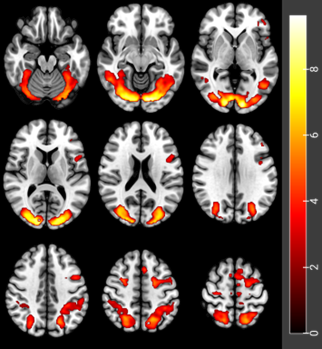
\includegraphics[clip, trim=0 0 0 0, width=\linewidth]{figs/AgeXCon_slice.png} % Replace with your image path
        \subcaption{XX: } \label{fig:b}
    \end{minipage}
    \caption{Age x Condition}
    \label{fig:AgexCon_Slice}
\end{figure}




\begin{figure}[ht]
    \centering
    \begin{minipage}{0.48\textwidth}
        \centering
        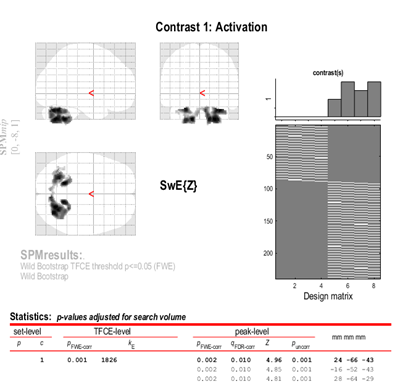
\includegraphics[clip, trim=0 0 0 0, width=\linewidth]{figs/OAcereb_spm.png} % Replace with your image path
        \subcaption{XX:} \label{fig:a}
    \end{minipage}
    % \hspace{\textwidth}
    \begin{minipage}{0.48\textwidth}
        \centering
        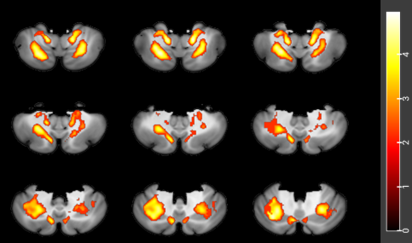
\includegraphics[clip, trim=0 0 0 0, width=\linewidth]{figs/OAcereb_slice.png} % Replace with your image path
        \subcaption{XX: } \label{fig:b}
    \end{minipage}
    \caption{OA cerebellum}
    \label{fig:OAcereb_slice}
\end{figure}



\begin{table}[h!]
\centering
\begin{tabular}{|l|l|c|c|c|c|c|}
\hline
\rowcolor[HTML]{D0D0D0} 
\textbf{Group}       & \textbf{Region}         & \textbf{pFWE-corr} & \textbf{kE} & \textbf{X} & \textbf{Y}  & \textbf{Z}  \\ \hline
Young adults         & NA                     & -                  & -           & -          & -           & -           \\ \hline
\multirow{3}{*}{Older adults} 
                    & Right Cerebellum 8     & 0.001              & 1826        & 24         & -66         & -43         \\ 
                    & Left Cerebellum 9      & -                  & -           & -16        & -52         & -43         \\ 
                    & Left Cerebellum 9      & -                  & -           & 28         & -64         & -29         \\ \hline
\end{tabular}
\caption{Group cerebellum results.}
\label{tab:Group cerebellum}
\end{table}



\begin{figure}[ht]
    \centering
    \begin{minipage}{0.48\textwidth}
        \centering
        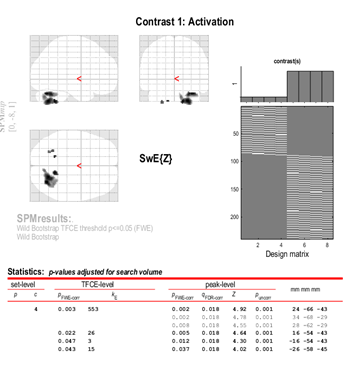
\includegraphics[clip, trim=0 0 0 0, width=\linewidth]{figs/OAYAcereb_spm.png} % Replace with your image path
        \subcaption{XX:} \label{fig:a}
    \end{minipage}
    % \hspace{\textwidth}
    \begin{minipage}{0.48\textwidth}
        \centering
        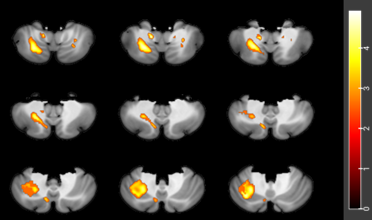
\includegraphics[clip, trim=0 0 0 0, width=\linewidth]{figs/OAYAcereb_slice.png} % Replace with your image path
        \subcaption{XX: } \label{fig:b}
    \end{minipage}
    \caption{OA > YA cerebellum}
    \label{fig:OAYAcereb_slice}
\end{figure}


\begin{table}[h!]
\centering
\begin{tabular}{|l|c|c|c|c|c|}
\hline
\rowcolor[HTML]{D0D0D0} 
\textbf{Region}              & \textbf{pFWE-corr} & \textbf{kE} & \textbf{X} & \textbf{Y} & \textbf{Z} \\ \hline
Right Cerebellum 8           & 0.003             & 553         & 24         & -66        & -43        \\ 
Right Cerebellum Crus I      & -                 & -           & 34         & -68        & -29        \\ 
Right Cerebellum 6           & -                 & -           & 28         & -62        & -29        \\ 
Right Cerebellum 9           & 0.022             & 26          & 16         & -54        & -43        \\ 
Right Cerebellum 9           & 0.047             & 3           & -16        & -54        & -43        \\ 
Left Cerebellum 8            & 0.043             & 15          & -26        & -58        & -45        \\ \hline
\end{tabular}
\caption{TFCE-level analysis results with MNI coordinates for identified brain regions for OA > YA cerebellum.}
\label{tab:tfce_oaya_cerebellum}
\end{table}


\begin{table}[h!]
\centering
\begin{tabular}{llrrrrrr}
\toprule
\multirow{2}{*}{}               & \multirow{2}{*}{}          & \textbf{Sum Sq}  & \textbf{Mean Sq} & \textbf{NumDF} & \textbf{DenDF} & \textbf{F value} & \textbf{Pr(>F)}          \\ 
\midrule
\multirow{3}{*}{\textbf{Short ISI}} 
                                & \textbf{Grp}              & 8496             & 4248             & 2              & 57             & 22.2194          & 7.339e-08 ***            \\
                                & \textbf{Cond}             & 112323           & 37441            & 3              & 171            & 195.8366         & < 2.2e-16 ***            \\
                                & \textbf{Grp:Cond}         & 7896             & 1316             & 6              & 171            & 6.8833           & 1.460e-06 ***            \\ 
\midrule
\multirow{3}{*}{\textbf{Long ISI}}
                                & \textbf{Grp}              & 11079            & 5539.3           & 2              & 57             & 23.6126          & 3.390e-08 ***            \\
                                & \textbf{Cond}             & 78785            & 26261.8          & 3              & 171            & 111.9464         & < 2.2e-16 ***            \\
                                & \textbf{Grp:Cond}         & 8475             & 1412.4           & 6              & 171            & 6.0208           & 9.814e-06 ***            \\ 
\bottomrule
\end{tabular}
\caption{Nback Accuracry statistical test results for Short and Long ISI conditions. Significance codes: 0 ‘***’ 0.001 ‘**’ 0.01 ‘*’ 0.05 ‘.’ 0.1 ‘ ’ 1.}
\label{tab:nback_accuracy}
\end{table}

\begin{figure}[ht]
    \centering
    \centering
    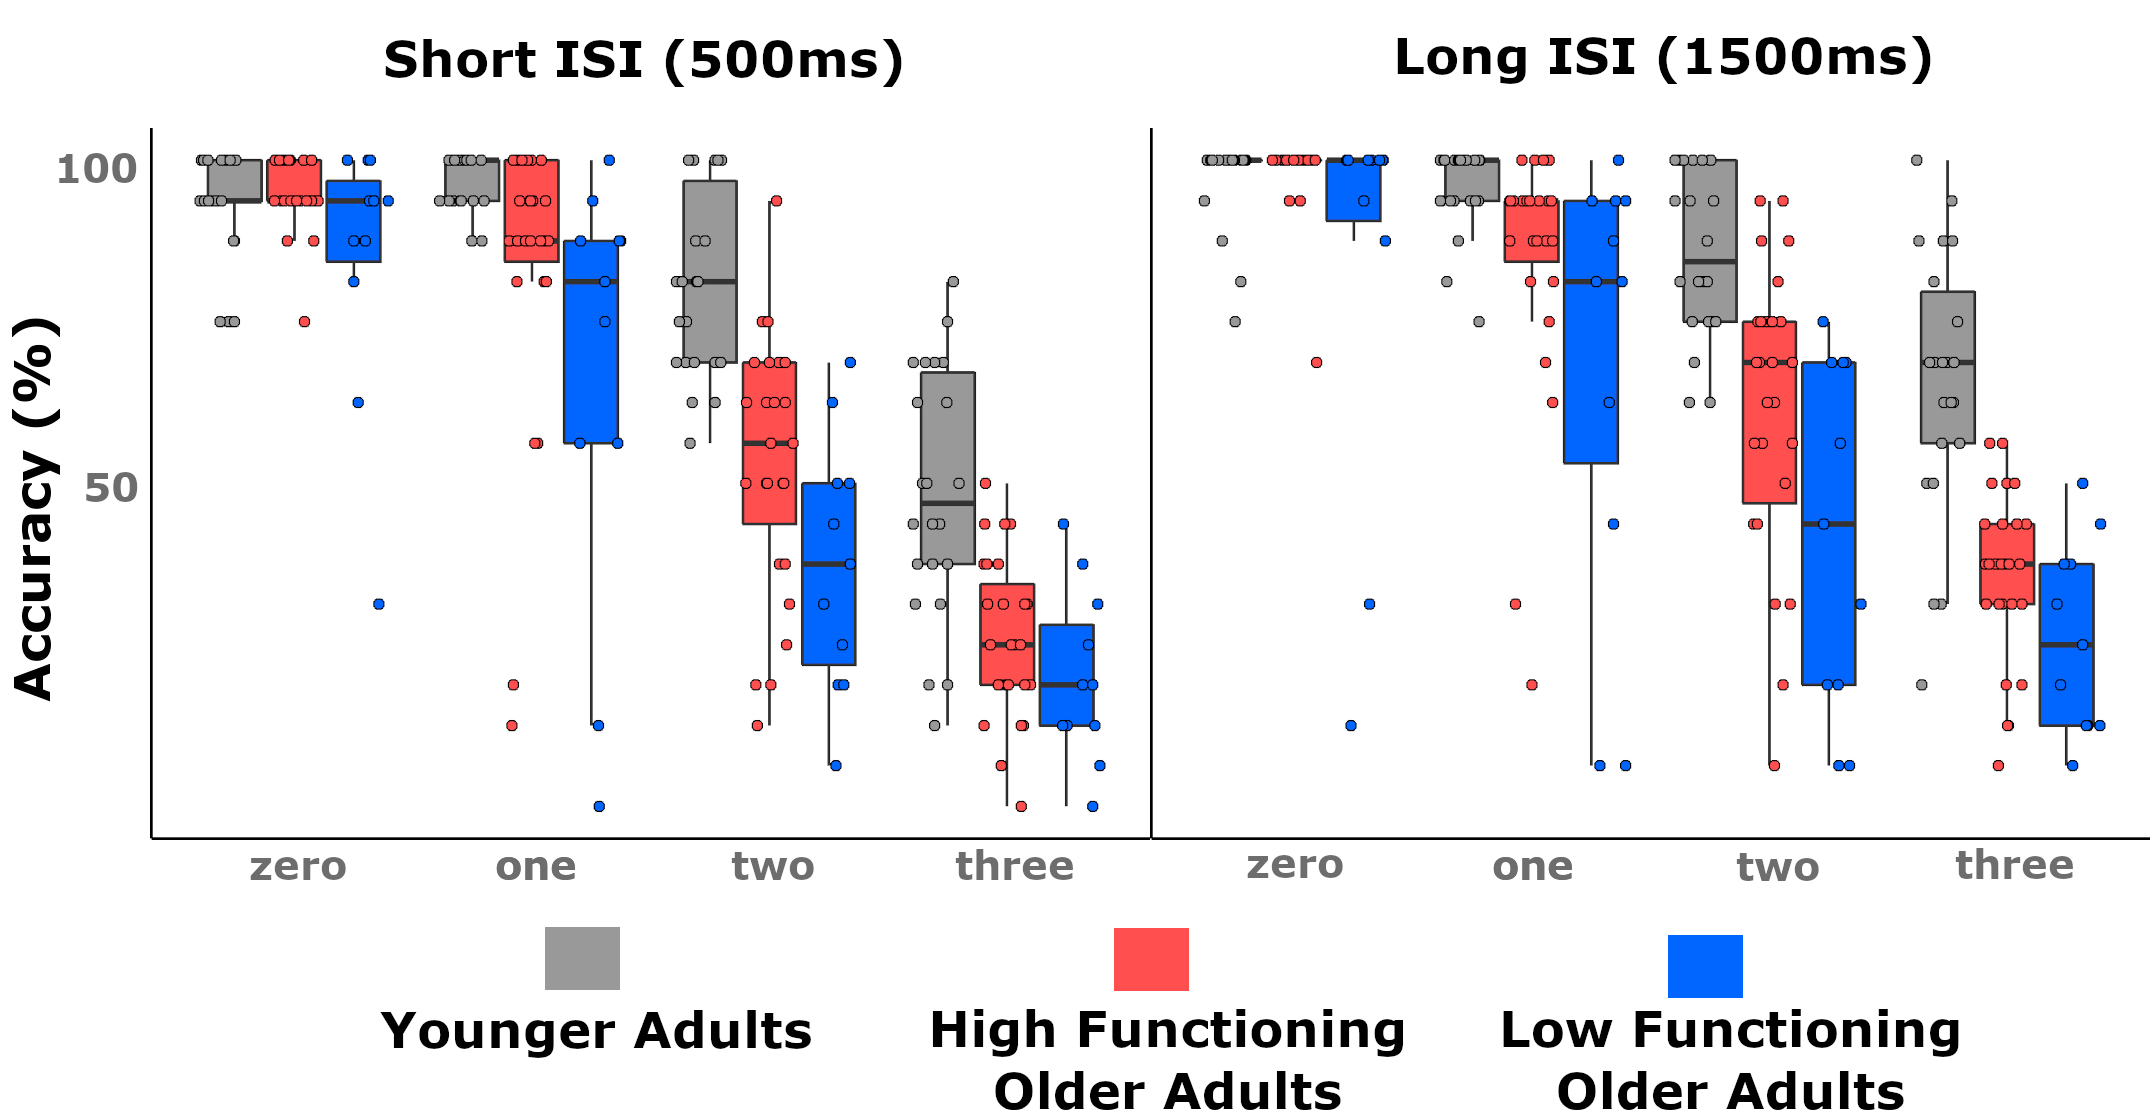
\includegraphics[clip, trim=0 0 0 0, width=\linewidth]{figs/nback_accuracy.png} % Replace with your image path
    \caption{Nback Accuracy}
    \label{fig:accuracry}
\end{figure}

\begin{table}[h!]
\centering
\begin{tabular}{llrrrrrr}
\toprule
\multirow{2}{*}{}               & \multirow{2}{*}{}          & \textbf{Sum Sq}  & \textbf{Mean Sq} & \textbf{NumDF} & \textbf{DenDF} & \textbf{F value} & \textbf{Pr(>F)}          \\ 
\midrule
\multirow{3}{*}{\textbf{Short ISI}} 
                                & \textbf{Grp}              & 152660           & 76330            & 2              & 57             & 8.0467           & 0.0008354 ***             \\
                                & \textbf{Cond}             & 549954           & 183318           & 3              & 171            & 19.3255          & 7.733e-11 ***             \\
                                & \textbf{Grp:Cond}         & 65099            & 10850            & 6              & 171            & 1.1438           & 0.3390838               \\ 
\midrule
\multirow{3}{*}{\textbf{Long ISI}}
                                & \textbf{Grp}              & 34256            & 17128            & 2              & 57.273          & 1.6007           & 0.2106                   \\
                                & \textbf{Cond}             & 571649           & 190550           & 3              & 168.989         & 17.8081          & 4.320e-10 ***             \\
                                & \textbf{Grp:Cond}         & 489859           & 81643            & 6              & 168.784         & 7.6301           & 2.929e-07 ***             \\ 
\bottomrule
\end{tabular}
\caption{Nback Reaction Time statistical test results for Short and Long ISI conditions. Significance codes: 0 ‘***’ 0.001 ‘**’ 0.01 ‘*’ 0.05 ‘.’ 0.1 ‘ ’ 1.}
\label{tab:reaction_tiem}
\end{table}

\begin{figure}[ht]
    \centering
    \centering
    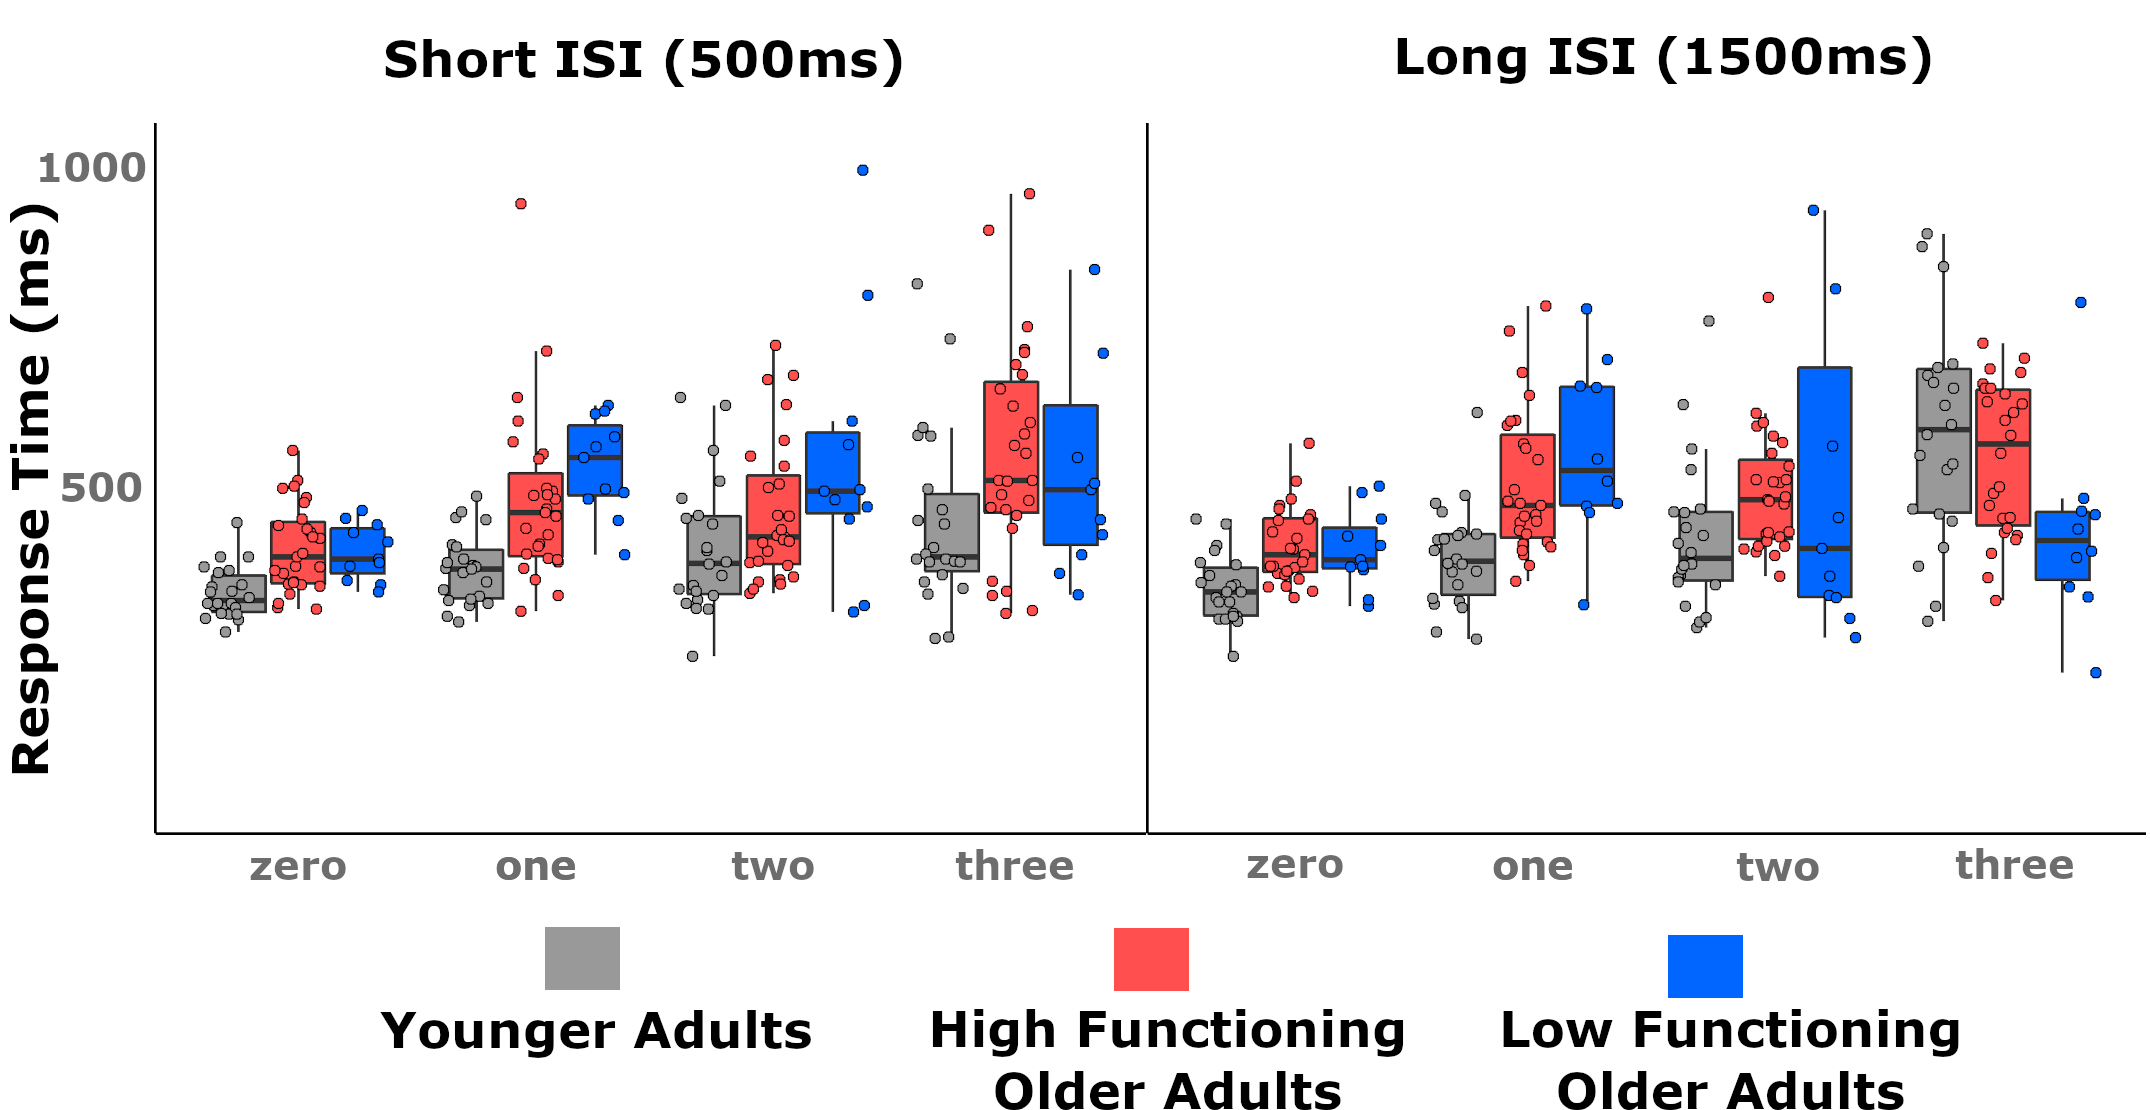
\includegraphics[clip, trim=0 0 0 0, width=\linewidth]{figs/nback_responseTime.png} % Replace with your image path
    \caption{Nback Response Time}
    \label{fig:responeTime}
\end{figure}



\end{document}




